\documentclass[11pt,table]{beamer}
\mode<presentation>
\usepackage{etex}
\usepackage{graphicx}
\usepackage{epstopdf}
\usepackage[english]{babel}
\usepackage{tabularx}
\usepackage{booktabs}
\usepackage{mathrsfs}
\usepackage{multicol}
\usepackage{bm}
\usepackage{subcaption}
\usepackage{wrapfig}
\usepackage{dcolumn}
\usepackage{threeparttable}
\usepackage{booktabs}
\usepackage{bbm}
\usepackage{amsmath,dsfont,listings}
\usepackage{amssymb}
\usepackage{rotating}
\usepackage{multirow}
\usepackage{tcolorbox}
\usepackage[authoryear]{natbib}
\usepackage{circledsteps}
\usepackage{qtree}

\usepackage{tikz}
\usetikzlibrary{arrows,decorations.pathmorphing,backgrounds,fit,positioning,shapes.symbols,chains}
\setbeamertemplate{section in toc}[sections numbered]
\setbeamertemplate{caption}[numbered]

\bibliographystyle{Econometrica}

\setbeamersize{text margin right=3.5mm, text margin left=7.5mm}  % text margin
\setbeamersize{sidebar width left=0cm, sidebar width right=0mm}
\setbeamertemplate{sidebar right}{}
\setbeamertemplate{sidebar left}{}

\definecolor{text-grey}{rgb}{0.45, 0.45, 0.45} % grey text on white background
\definecolor{bg-grey}{rgb}{0.66, 0.65, 0.60} % grey background (for white text)
\definecolor{fu-blue}{RGB}{0, 51, 102} % blue text
\definecolor{fu-green}{RGB}{153, 204, 0} % green text
\definecolor{fu-red}{RGB}{204, 0, 0} % red text (used by \alert)
\definecolor{BrewerBlue}{HTML}{377EB8} % Define Brewer Blue
\definecolor{BrewerRed}{HTML}{E41A1C}  % Define Brewer Red

\setbeamertemplate{frametitle}{%
    \vskip-30pt \color{text-grey}\large%
    \begin{minipage}[b][23pt]{\textwidth}%
    \flushleft\insertframetitle%
    \end{minipage}%
}

\setbeamertemplate{navigation symbols}{} 

%%% begin title page
\setbeamertemplate{title page}{
\vskip2pt\hfill
\vskip19pt\hskip3pt

% set the title and the author
\vskip4pt
\parbox[top][1.35cm][c]{11cm}{\LARGE\color{text-grey} \textcolor{red1}{RL}earning:\\[1ex] \inserttitle \\[1ex] \small \quad \\[3ex]}
\vskip17pt
\parbox[top][1.35cm][c]{11cm}{\small Unit 1-2: \insertsubtitle \\[2ex] \insertauthor \\[1ex]}
}
%%% end title page

%%% colors
\usecolortheme{lily}
\setbeamercolor*{normal text}{fg=black,bg=white}
\setbeamercolor*{alerted text}{fg=fu-red}
\setbeamercolor*{example text}{fg=fu-green}
\setbeamercolor*{structure}{fg=fu-blue}

\setbeamercolor*{block title}{fg=white,bg=black!50}
\setbeamercolor*{block title alerted}{fg=white,bg=black!50}
\setbeamercolor*{block title example}{fg=white,bg=black!50}

\setbeamercolor*{block body}{bg=black!10}
\setbeamercolor*{block body alerted}{bg=black!10}
\setbeamercolor*{block body example}{bg=black!10}

\setbeamercolor{bibliography entry author}{fg=fu-blue}
\setbeamercolor{bibliography entry journal}{fg=text-grey}
\setbeamercolor{item}{fg=fu-blue}
\setbeamercolor{navigation symbols}{fg=text-grey,bg=bg-grey}
%%% end colors

%%% headline
\setbeamertemplate{headline}{
\vskip30pt
}
%%% end headline

%%% footline
\newcommand{\footlinetext}{
%\insertshortinstitute, \insertshorttitle, \insertshortdate
}
\setbeamertemplate{footline}{
\vskip2pt
\hfill \raisebox{-1pt}{\usebeamertemplate***{navigation symbols}}
\hfill \insertframenumber\hspace{10pt}
\vskip4pt
}
%%% end footline

%%% settings for listings package
\lstset{extendedchars=true, showstringspaces=false, basicstyle=\footnotesize\sffamily, tabsize=2, breaklines=true, breakindent=10pt, frame=l, columns=fullflexible}
\lstset{language=Java} % this sets the syntax highlighting
\lstset{mathescape=true} % this switches on $...$ substitution in code
% enables UTF-8 in source code:
\lstset{literate={ä}{{\"a}}1 {ö}{{\"o}}1 {ü}{{\"u}}1 {Ä}{{\"A}}1 {Ö}{{\"O}}1 {Ü}{{\"U}}1 {ß}{\ss}1}
%%% end listings

\usepackage{concmath}
\usepackage{xcolor}
\definecolor{red1}{RGB}{206, 17, 38}
\definecolor{blue1}{RGB}{16, 118, 208}
\definecolor{gray1}{RGB}{117, 115, 115}
\usepackage{hyperref}


\newtheorem{proposition}{Proposition}
\newtheorem{assumption}{Definition}

\title[]{Short guides to reinforcement learning}
\subtitle[]{Greedy, $\varepsilon$-greedy, decaying $\varepsilon$-greedy}
\author[D. Rostam-Afschar]{\textcolor{gray1}{Davud Rostam-Afschar (Uni Mannheim)}}
\date[]{\today}
\subject{Econometrics}
\renewcommand{\footlinetext}{\insertshortinstitute, \insertshorttitle, \insertshortdate}
\hypersetup{
    bookmarks=false,
    unicode=false,
    pdftoolbar=false,
    pdffitwindow=true,
    pdftitle={Reinforcement Learning for Business, Economics, and Social Sciences: \insertsubtitle},
    pdfauthor={Davud Rostam-Afschar},
    pdfsubject={Reinforcement Learning},
    pdfkeywords={reinforcement learning, Multi-Armed Bandits},
    pdfnewwindow=true,
}
\def\sym#1{\ifmmode^{#1}\else\(^{#1}\)\fi}

\begin{document}

\begin{frame}[plain]
  \titlepage
\end{frame}

% --------------------------------------------------- Slide --
%\begin{frame}
	%\frametitle{Content}
	%\tableofcontents[]
%\end{frame}

\section{epsilon-first}
{
\setbeamercolor{background canvas}{bg=BrewerBlue}
\begin{frame}
\centering
\Huge
\textcolor{white}{How much to learn\\ about the average return?}
\thispagestyle{empty}
\end{frame}
}
{
\setbeamercolor{background canvas}{bg=BrewerBlue}
\begin{frame}
\centering
\Huge
\textcolor{white}{$\varepsilon$-First + Greedy Policy}
\thispagestyle{empty}
\end{frame}
}


\begin{frame}\frametitle{$\varepsilon$-First + Greedy Policy}
\renewcommand{\baselinestretch}{1}
\begin{figure}
    \centering
    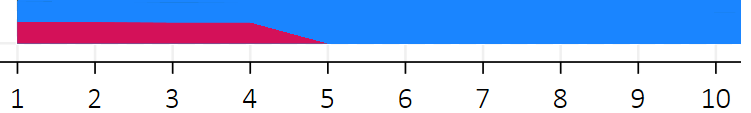
\includegraphics[width=0.9\linewidth]{figures/epsilon first 2.png}
\end{figure}
\begin{itemize}
    \item Epsilon-first is widely known as A/B testing
    \item Often applied to two-armed bandits
    %\item The first $\varepsilon$ share of trials serve as exploration or burn-in phase
    %\item Researchers assign a uniform share of participants to each arm
    %\item Estimate each arm’s outcome
    %\item In the remaining $(1-\varepsilon)$ share of trials (exploitation phase)\\
    %$\rightarrow$ only the arm with the best empirical estimate is selected
\end{itemize}

\end{frame}


\begin{frame}{Fixed Exploration Period + Greedy}
\begin{figure}
    \centering
    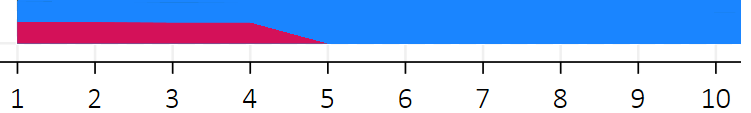
\includegraphics[width=0.9\linewidth]{figures/epsilon first 2.png}
\end{figure}
    \begin{tcolorbox}[colframe=black, boxrule=1pt, sharp corners, ]
        \begin{enumerate}\small 
            \item Allocate a fixed time period to exploration, during which you try all bandits uniformly at random.\pause
            \item Estimate mean rewards for all actions:
            \[
                Q_t(a) = \frac{1}{N_t(a)} \sum_{i=1}^{t-1} R_i \cdot \mathds{1}(A_i = a)
            \]\vspace*{-2ex}\pause
            \item Select the action that is optimal for the estimated mean rewards (breaking ties randomly):
            \[
                a_t = \arg\max_{a \in \mathcal{A}} Q_t(a)
            \]\vspace*{-2.5ex}\pause
            \item Repeat step 3 for all future time steps.
        \end{enumerate}
    \end{tcolorbox}
\end{frame}


\section{(Decaying) epsilon-greedy}
{
\setbeamercolor{background canvas}{bg=BrewerBlue}
\begin{frame}
\centering
\Huge
\textcolor{white}{$\varepsilon$-greedy}
\thispagestyle{empty}
\end{frame}
}

\begin{frame}\frametitle{$\varepsilon$-greedy}
\renewcommand{\baselinestretch}{1}
\begin{figure}
    \centering
    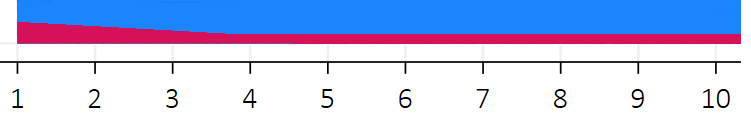
\includegraphics[width=0.9\linewidth]{figures/epsilon greedy 2.png}
\end{figure}
\begin{itemize}
    \item Explores for the entire number of trials of the experiment
    \item simple and popular heuristic \citep{sutton2018reinforcement, Bubeck2012, Burtini2015}%\item Selects best treatment for share $(1-\varepsilon)$ of all trials
    %\item Share can be constant or decreasing
    %\item Assigns all treatment arms with equal probability for share $\varepsilon$
    %\item Even after having learned about the average outcome of each arm, constant epsilon-greedy explores some epsilon fraction of the trials\\
    %$\rightarrow$ asymptotically no convergence to optimal arm
\end{itemize}

\end{frame}


\begin{frame}{$\varepsilon$-greedy}
\textbf{Idea:} Exploit, but explore a random arm with $\varepsilon$ probability

\vspace{1em}
\begin{enumerate}
    \item \textbf{Initial phase:} Try each arm and observe the rewards\pause

    \item \textbf{For each round } $t = n+1, \ldots, T$:
    \begin{itemize}
        \item Estimate action values from \emph{sample averages} for each arm $a$:
\begin{align*}
        Q_{t}(a) &= \frac{\text{sum of rewards when }a\text{ taken prior to }t}{\text{number of times }a\text{ taken prior to }t}=\frac{\sum_{i=1}^{t-1} R_i \mathds{1}(A_i=a)}{\sum_{i=1}^{t-1} \mathds{1}(A_i=a)}
\end{align*}
        \pause
        \item With probability $1 - \varepsilon$, play the arm with highest $Q_{t}(a)$\pause
        \item With probability $\varepsilon$, choose an arm uniformly at random
    \end{itemize}
\end{enumerate}
\end{frame}


\begin{frame}{A Simple $\varepsilon$-Greedy Bandit Algorithm}
\begin{figure}
    \centering
    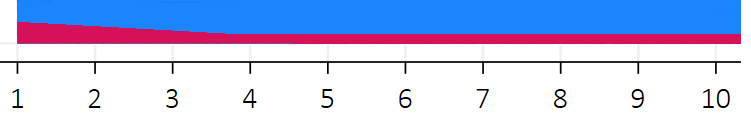
\includegraphics[width=0.9\linewidth]{figures/epsilon greedy 2.png}
\end{figure}
\begin{tcolorbox}[colframe=black, boxrule=1pt, sharp corners]
\begin{itemize}\small
    \item \textbf{Initialize:} For each action $a = 1$ to $k$:
    \begin{itemize}
        \item $Q(a) \gets 0$ \hfill 
        \item $N(a) \gets 0$ \hfill 
    \end{itemize}
    
    \item \textbf{Loop forever:}
    \begin{itemize}\small\vspace*{-2.5ex}
		 \item[]
       \[
        A = 
        \begin{cases}
            \arg\max_a Q(a) & \text{with probability } 1 - \varepsilon \\
            \text{random action} & \text{with probability } \varepsilon
        \end{cases}
        \]
        \item Receive reward: $R \gets \text{bandit}(A)$
        \item Update count: $N(A) \gets N(A) + 1$
        \item Update estimate:\vspace*{-2ex}
        \[
        Q(A) \gets Q(A) + \frac{1}{N(A)} (R - Q(A))
        \]
    \end{itemize}
\end{itemize}
\end{tcolorbox}

\end{frame}

\section{Exploration vs Exploitation}
{
\setbeamercolor{background canvas}{bg=BrewerBlue}
\begin{frame}
\centering
\Huge
\textcolor{white}{Exploration vs Exploitation}
\thispagestyle{empty}
\end{frame}
}




\begin{frame}{Regrets of Greedy Policies}

\centering
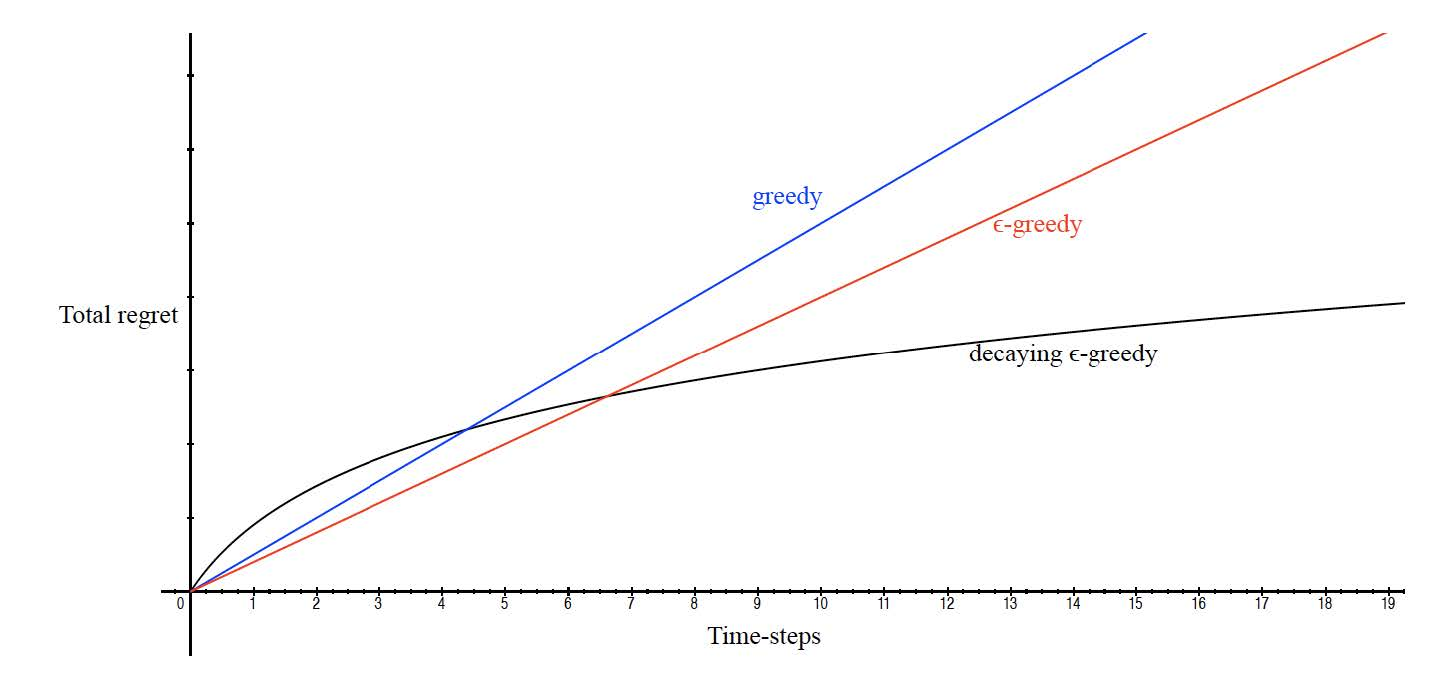
\includegraphics[width=0.8\textwidth]{figures/regrets of greedy policies.jpg}


\scriptsize\hfill\textit{Source: David Silver}
\vspace{.5em}

\centering
\renewcommand{\arraystretch}{1.2} % Increase row height

\begin{tabular}{p{0.30\textwidth} p{0.30\textwidth} p{0.30\textwidth}}
\footnotesize
\textbf{Greedy Policy} & \textbf{$\varepsilon$-Greedy} & \textbf{Decaying $\varepsilon$} \\
\toprule
Never explores & Always explores with probability $\varepsilon$ & Decreases exploration over time \\
Locks on sub-optimal policy & See decomposition lemma & Requires careful tuning \\
\emph{Linear} regret & \emph{Linear} regret & \emph{Sub-Linear} regret \\
\bottomrule
\end{tabular}

\vspace{1em}

\centering
\footnotesize
$\Rightarrow$ \textit{Convergence rate depends on $\varepsilon$ choice \citep{auer2002finite}}
\normalsize

\end{frame}



\begin{frame}{Theoretical Guarantees}

  \[
  \text{Loss}_T = \sum_{t=1}^{T}\text{loss}_t =   \sum_{a \in \mathcal{A}} \mathbb{E}\left[\sum_{i=1}^{t-1}\mathds{1} \{A_i = a\}\right] (r^* - q(a)) 
  \]


    \begin{itemize}
        \item When $\varepsilon$ is constant, probability to explore in each step $t$ is $\varepsilon$
				\item Each action is selected with probability $1/\mathcal{A}$
				\item Probability of choosing a suboptimal action $\mathbb{P}\left(a_{t} \neq a^{*}\right) = \varepsilon/\mathcal{A}$
				\item Expected regret: $\operatorname{loss}_{t}\geq\frac{\varepsilon}{\mathcal{A}}\sum_{a\in\mathcal{A}}(r^* - q(a))$\\[2ex]\pause
				\item Expected number of times action $a$ is selected due to exploration over $T$ steps $\frac{\varepsilon T}{\mathcal{A}}$
				\item Expected cumulative regret: $\operatorname{Loss}_{T} = \frac{\varepsilon T}{\mathcal{A}}\sum_{a\in\mathcal{A}}(r^* - q(a)) =\mathcal{O}(T)$
\item  \textcolor{red1}{Linear regret}
\end{itemize}
\end{frame}

\begin{frame}{Theoretical Guarantees}
	

    \begin{itemize}
\item When $\varepsilon \propto 1 / t$

\begin{itemize}
\item   For large enough $t: \mathbb{P}\left(a_{t} \neq a^{*}\right) \approx \varepsilon_{t}=\mathcal{O}(1 / t)$
\item   Expected cumulative regret: $\operatorname{Loss}_{T} \approx \sum_{t=1}^{T} 1 / t  =\mathcal{O}(\log T)$
\item   \textcolor{red1}{Logarithmic regret}
    \end{itemize}
    \end{itemize}
\end{frame}


\begin{frame}[t,allowframebreaks
]%\nocite{*}
\frametitle{References}
\small
\bibliography{bib}
\end{frame}
\section{Takeaways}
{
\setbeamercolor{background canvas}{bg=BrewerBlue}
\begin{frame}
\centering
\Huge
\textcolor{white}{Takeaways}
\thispagestyle{empty}
\end{frame}
}

\begin{frame}{What does the $\varepsilon$-greedy algorithm?}
\begin{itemize}
    \item $\varepsilon$-greedy algorithm balances exploration and exploitation
		\item With probability $\varepsilon$, it explores randomly
    \item With $1 - \varepsilon$, it chooses action with highest empirical mean
    \item A constant $\varepsilon$ ensures ongoing exploration but leads to linear regret
    \item A decaying $\varepsilon$ enables convergence to the optimal arm and may achieve logarithmic regret
\end{itemize}



\end{frame}


\end{document}
